\documentclass[a4paper, 12pt]{report}

\usepackage[dvipsnames]{xcolor}

%%%%%%%%%%%%%%%%
% Set Variables %
%%%%%%%%%%%%%%%%

\def\useItalian{0}  % 1 = Italian, 0 = English

\def\courseName{Advanced Algorithms}

\def\coursePrerequisites{\begin{itemize} \item Progettazione degli Algoritmi \end{itemize}}

\def\book{TODO}

% \def\authorName{Simone Bianco}
% \def\email{bianco.simone@outlook.it}
% \def\github{https://github.com/Exyss/university-notes}
% \def\linkedin{https://www.linkedin.com/in/simone-bianco}

\def\authorName{Alessio Bandiera}
\def\email{alessio.bandiera02@gmail.com}
\def\github{https://github.com/aflaag-notes}
\def\linkedin{https://www.linkedin.com/in/alessio-bandiera-a53767223}

%%%%%%%%%%%%
% Packages %
%%%%%%%%%%%%

\usepackage{../../packages/Nyx/nyx-packages}
\usepackage{../../packages/Nyx/nyx-styles}
\usepackage{../../packages/Nyx/nyx-frames}
\usepackage{../../packages/Nyx/nyx-macros}
\usepackage{../../packages/Nyx/nyx-title}
\usepackage{../../packages/Nyx/nyx-intro}

%%%%%%%%%%%%%%
% Title-page %
%%%%%%%%%%%%%%

\logo{../../packages/Nyx/logo.png}

\if\useItalian1
    \institute{\curlyquotes{\hspace{0.25mm}Sapienza} Università di Roma}
    \faculty{Ingegneria dell'Informazione,\\Informatica e Statistica}
    \department{Dipartimento di Informatica}
    \ifdefined\book
        \subtitle{Appunti integrati con il libro \book}
    \fi
    \author{\textit{Autore}\\\authorName}
\else
    \institute{\curlyquotes{\hspace{0.25mm}Sapienza} University of Rome}
    \faculty{Faculty of Information Engineering,\\Informatics and Statistics}
    \department{Department of Computer Science}
    \ifdefined\book
        \subtitle{Lecture notes integrated with the book \book}
    \fi
    \author{\textit{Author}\\\authorName}
\fi


\title{\courseName}
\date{\today}

% \supervisor{Linus \textsc{Torvalds}}
% \context{Well, I was bored\ldots}

\addbibresource{./references.bib}

%%%%%%%%%%%%
% Document %
%%%%%%%%%%%%

\begin{document}
    \maketitle

    % The following style changes are valid only inside this scope 
    {
        \hypersetup{allcolors=black}
        \fancypagestyle{plain}{%
        \fancyhead{}        % clear all header fields
        \fancyfoot{}        % clear all header fields
        \fancyfoot[C]{\thepage}
        \renewcommand{\headrulewidth}{0pt}
        \renewcommand{\footrulewidth}{0pt}}

        \romantableofcontents
    }

    \introduction

    %%%%%%%%%%%%%%%%%%%%%

    \chapter{TODO}

    \section{TODO}

    \subsection{The Max Cut problem}

    The \tbf{Max Cut problem} --- in the unweighted case --- is a classic combinatorial optimization problem in the branch of \href{https://en.wikipedia.org/wiki/Graph_theory}{graph theory}, in which we seek to partition the vertices of an undirected graph into two disjoint subsets while maximizing the number of edges that have endpoints in both subsets. More formally, we will define a \tbf{cut} of a graph as follows.

    \begin{frameddefn}{Cut of a graph}
        Given an undirected graph $G = (V, E)$, and a subset of its vertices $S \subseteq V$, the \tbf{cut} induced by $S$ on $G$ is defined as follows $$\mathrm{cut}(S) := \{e \in E \mid \abs{S \cap e} = 1\}$$
    \end{frameddefn}

    Note that in the definition above we are defining the cut of a graph through the intersection between a set of vertices $S$ and edges in $E$; this is because, in the undirected case, we will consider the edges of a graph $G = (V, E)$ as sets of 2 elements $$E = \{\{u, v\} \mid u, v \in V\}$$ Therefore, given a set of vertices $S$, the cut induced by $S$ is simply the set of edges that have only one endpoint in $S$ (implying that the other one will be in $V - S$).

    \begin{figure}[H]
        \centering
        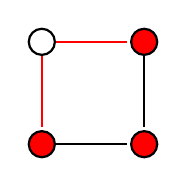
\begin{tikzpicture}[-,>=stealth,shorten >=1pt,auto,node distance=1.3cm, thick,main node/.style={scale=0.9,circle,draw,font=\sffamily\normalsize}]

            \node[circle, draw]  (1) []{};
            \node[circle, draw, fill=red]  (2) [below of = 1]{};
            \node[circle, draw, fill=red]  (3) [right of = 1]{};
            \node[circle, draw, fill=red]  (4) [below of = 3]{};

            % \path[every node/.style={font=\sffamily\small}]

            \draw[-] (1) [red] to (2);
            \draw[-] (1) [red] to (3);
            \draw[-] (2) to (4);
            \draw[-] (3) to (4);

            ;
        \end{tikzpicture}
        \caption{Given the set of red vertices $S$, the green edges represent $\mathrm{cut}(S)$.}
    \end{figure}

    With this definition, we can introduce the \tbf{Max Cut} problem, which is defined as follows.

    \begin{frameddefn}{Max Cut problem}
        Given an undirected graph $G = (V, E)$, determine the set $S \subseteq V$ that maximizes $\abs{\mathrm{cut}(S)}$.
    \end{frameddefn}

    Although this problem is known to be \textsf{APX-Hard} \cite{maxcut}, approximation algorithms and heuristic methods like greedy algorithms and local search are commonly used to find near-optimal solutions.

    For now, we present the following \tbf{randomized algorithm}, which provides a straightforward $\frac{1}{2}$-approximation for the Max Cut problem. This algorithm runs in polynomial time and achieves the approximation guarantee with high probability.

    \begin{framedalgo}{Random Cut}
        Given an undirected graph $G = (V, E)$, the algorithm returns a cut of the graph. \\
        \hrule

        \quad
        \begin{algorithmic}[1]
            \Function{RandomCut}{$G$}
                \State $S := \varnothing$
                \For{$v \in V$}
                    \State Let $c_v$ be the outcome of the flip of an independent fair coin
                    \If{$c_v == \mathrm{heads}$}
                        \State $S = S \cup \{v\}$
                    \EndIf
                \EndFor
                \State \textbf{return} $S$
            \EndFunction
        \end{algorithmic}
    \end{framedalgo}

    Note that this algorithm does not care about the structure of the graph in input, since the output is completely determined by the coin flips performed in the \texttt{for} loop. Now we will prove that this algorithm is a correct \tbf{expected $\frac{1}{2}$-approximation} of the Max Cut problem.
    
    \begin{framedthm}[label={expected random cut}]{Expected approximation ratio of \textsc{RandomCut}}
        Let $G= (V, E)$ be a graph, and let $S^*$ be an optimal solution to the Max Cut problem on $G$. Then, given $S = \textsc{RandomCut}(G)$, it holds that $$\mathbb E [\abs{\mathrm{cut}(S)}] \ge \dfrac{\abs{\mathrm{cut}(S^*)}}{2}$$
    \end{framedthm}

    \begin{proof}
        By definition, note that $$\forall e \in E \quad e \in \mathrm{cut}(S) \iff \abs{S \cap e} = 1$$ Consider an edge $e = \{v, w\} \in E$; then, by definition $$\{v, w\} \in \mathrm{cut}(S) \iff (v \in S \land w \notin S) \lor (v \notin S \land w \in S)$$ and let $\xi_1$ and $\xi_2$ be these last two events respectively. Then $$\Pr[\xi_1] = \Pr[c_v = \mathrm{heads} \land c_w = \mathrm{tails}]$$ by definition of the algorithm, and by independence of the flips of the fair coins we have that $$\Pr[\xi_1] = \Pr[c_v = \mathrm{heads}] \cdot \Pr[c_w = \mathrm{tails}] = \dfrac{1}{2} \cdot \dfrac{1}{2} = \dfrac{1}{4}$$ Analogously, we can show that $$\Pr[\xi_2] = \dfrac{1}{4}$$ This implies that $$\Pr[e \in \mathrm{cut}(S)] = \Pr[\xi_1 \lor \xi_2] = \Pr[\xi_1] + \Pr[\xi_2] - \Pr[\xi_1 \land \xi_2] = \dfrac{1}{4} + \dfrac{1}{4} - 0 = \dfrac{1}{2}$$ Hence, we have that $$\mathbb E [\abs{\mathrm{cut}(S)}] = \sum_{e \in E}{1 \cdot \Pr[e \in \mathrm{cut}(S)]} = \dfrac{\abs E}{2} \ge \dfrac{\abs{\mathrm{cut}(S^*)}}{2}$$ where the last inequality directly follows from the definition of cut of a graph.
    \end{proof}

    As previously mentioned, this algorithm has an \tbf{expected approximation ratio} of $\frac{1}{2}$, which implies that it may return very bad solutions in some cases, depending on the outcomes of the coin flips. However, thanks to the following algorithm, we can actually transform the \tbf{guarantee of expectations} into a \tbf{guarantee of high probability}.

    \begin{framedalgo}{$t$-times Random Cut}
        Given an undirected graph $G = (V, E)$ and an integer $t > 0$, the algorithm returns a cut of the graph. \\
        \hrule

        \quad
        \begin{algorithmic}[1]
            \Function{$t$-timesRandomCut}{$G$, $t$}
                \For{$i \in [t]$}
                    \State $S_i := \textsc{RandomCut}(G)$
                \EndFor
                \State \textbf{return} $S \in \argmax_{i \in [t]}{\abs{\mathrm{cut}(S_i)}}$
            \EndFunction
        \end{algorithmic}
    \end{framedalgo}

    The algorithm above simply runs the \textsc{RandomCut} algorithm $t$ times, and returns the set $S_i$ that maximizes the cut, among all the various $S_1, \ldots, S_t$. The following theorem will show that a \tit{reasonable number} of runs of the \textsc{RandomCut} algorithm suffices in order to almost certainly obtain a $\approx \frac{1}{2}$-approximation of any optimal solution.

    \begin{framedthm}{}
        Let $G= (V, E)$ be a graph, and let $S^*$ be an optimal solution to the Max Cut problem on $G$. Then, given $S = \textsc{$t$-timesRandomCut}(G, t)$, it holds that $$\Pr \sbk{\abs{\mathrm{cut}(S)} > \dfrac{1 - \varepsilon}{2} \abs{\mathrm{cut}(S^*)}} > 1 - \delta$$ where $t = \frac{2}{\varepsilon} \ln {\frac{1}{\delta}}$ and $0 < \varepsilon, \delta < 1$.
    \end{framedthm}
    
    \begin{proof}
        For each $i \in [t]$, let $C_i := \abs{\mathrm{cut}(S_i)}$ for each $S_i$ defined by the algorithm, and let $N_i := \abs E - C_i$. Let $0 < \varepsilon < 1$; since $N_i$ is a non-negative random variable, by \href{https://en.wikipedia.org/wiki/Markov%27s_inequality}{Markov's inequality} we have that $$\Pr[N_i \ge (1 + \varepsilon) \mathbb E [N_i]] \le \dfrac{1}{1 + \varepsilon} = 1 - \dfrac{\varepsilon}{1 + \varepsilon} \le 1 - \dfrac{\varepsilon}{2}$$ In particular, this inequality can be rewritten as follows:
        \begin{equation*}
            \begin{split}
                1 - \dfrac{\varepsilon}{2} &\ge \Pr[N_i \ge (1 + \varepsilon) \mathbb E [N_i]] \\
                                           &= \Pr[\abs E - C_i \ge (1 + \varepsilon)(\abs E - \mathbb E [C_i])] \\
                                           &= \Pr[- \varepsilon \abs E \ge C_i - (1 + \varepsilon) \mathbb E [C_i]]
            \end{split}
        \end{equation*}
        As shown in the proof of \cref{expected random cut}, we know that $\mathbb E [C_i] = \frac{\abs E}{2}$, therefore
        \begin{equation*}
            \begin{split}
                1 - \dfrac{\varepsilon}{2} &\ge \Pr[- \varepsilon \abs E \ge C_i - (1 + \varepsilon) \mathbb E [C_i]] \\
                                           &= \Pr \sbk{- \varepsilon \abs E \ge C_i - \dfrac{1 + \varepsilon}{2} \abs E} \\
                                           &= \Pr \sbk{- \varepsilon \dfrac{\abs E}{2} \ge C_i - \dfrac{\abs E}{2}} \\
                                           &= \Pr \sbk{\dfrac{1 - \varepsilon}{2} \abs E\ge C_i} \\
                                           &= \Pr \sbk{(1 - \varepsilon) \mathbb E[C_i] \ge C_i} \\
            \end{split}
        \end{equation*}
        Note that the event in the last probability, namely $$\abs{\mathrm{cut}(S_i)}  \le (1 - \varepsilon) \mathbb E [\abs{\mathrm{cut}(S_i)}]$$ corresponds to a \curlyquotes{bad} solution, i.e. one whose cardinality is at most $(1 - \varepsilon)$-th of the expected value.

        By definition of the algorithm, each of the $t$ runs of the \textsc{RandomCut} algorithm is independent from the others, therefore the probability of \tit{all} the solutions $S_1, \ldots, S_t$ being \curlyquotes{bad} is bounded by $$\Pr[\forall i \in [t]  \quad C_i \le (1 - \varepsilon) \mathbb E [C_i]] = \prod_{i = 1}^t{\Pr[C_i \le (1 - \varepsilon)\mathbb E[C_i]]} \le \rbk{1 - \dfrac{\varepsilon}{2}}^t$$

        Using the fact that $$\forall x \in \R \quad 1 - x \le e^{-x} \implies 1 - \frac{\varepsilon}{2} \le e^{- \frac{\varepsilon}{2}}$$ we have that $$\Pr[\forall i \in [t] \quad C_i \le (1 - \varepsilon) \mathbb E[C_i]] \le \rbk{1 - \dfrac{\varepsilon}{2}}^t \le e^{- \frac{\varepsilon}{2} \cdot t} = e^{- \ln {\frac{1}{\delta}}} = \delta$$

        Therefore, the probability that at least one among $S_1, \ldots, S_t$ is a \curlyquotes{good} solution is bounded by $$\Pr[\exists i \in [t] \quad C_i > (1 - \varepsilon) \mathbb E [C_i]] = 1 - \Pr[\forall i \in [t] \quad C_i \le (1 - \varepsilon) \mathbb E [C_i]] \ge 1 - \delta$$

        placeholder \todo{last part}
    \end{proof}

    Note that this result is \tit{very powerful}: for instance, if $\varepsilon = \delta = 0.1$, we get that $$\Pr[\abs{\mathrm{cut}(S)} > 0.45 \cdot \abs{\mathrm{cut}(S^*)}] \ge 0.9$$ and $t \approx 46$, meaning that we just need to run the \textsc{RandomCut} algorithm approximately 46 times in order to get a solution that is better than a $0.45$-approximation with $90\%$ probability.

    \printbibliography % UNCOMMENT FOR BIBLIOGRAPHY

\end{document}
